The goal of our work is to analyze a web API statically and from this analysis, 
without deploying or running the web API, 
to accurately estimate an upper bound on its execution time. With such a prediction,
we can provide a performance SLA to the users (human or 
programmatic) of the web API under development to help others reason its performance
and use in their web APIs -- something that is not possible today.
For general purpose applications, such worst case execution time analysis has been shown
by numerous researchers to be extremely complex and challenging to achieve for all but 
very simple codes or very specific domains.
To overcome these challenges, we take inspiration from the latter and exploit 
the development and deployment model of PaaS systems for web API execution to enable 
our analysis and accurate performance predictions.

First, PaaS systems require developers
to implement web APIs using a predefined set of 
programming interfaces. When considered as a
collection, we shall refer to these programming interfaces as the cloud software development 
kit or the \textit{cloud SDK}. We refer to the individual member interfaces of the cloud SDK
as \textit{cloud SDK interfaces}, and their constituent operations are referred to as \textit{cloud SDK operations}.

App Engine, for example, provides several cloud SDKs; one for each
programming language supported (Java, Python, Go etc). Each SDK consists of
several cloud SDK interfaces. Table~\ref{tab:gae_cloud_sdk} lists some of them.
Each individual interface is comprised of several cloud SDK operations. For instance, the 
datastore interface of App Engine provides operations for saving an entity (a data object),
deleting an entity, and querying the datastore to read one or more entities.

\begin{table}[htdp]
\caption{Google App Engine cloud SDK interfaces}
\begin{center}
\begin{tabular}{|c|p{5cm}|}
\hline
Cloud SDK Interface & Functionality \\ \hline
datastore & Reading and writing data to a highly scalable database with some transaction support. \\ \hline
memcache & In-memory caching of data for faster access.\\ \hline
users & User session management (login and logout)\\ \hline
blobstore & Reading and writing large chunks (blobs) of uninterpreted bytes.\\ \hline
task queue & Scheduling periodic and background jobs.\\ \hline
\end{tabular}
\end{center}
\label{tab:gae_cloud_sdk}
\end{table}

\begin{figure}
\centering
%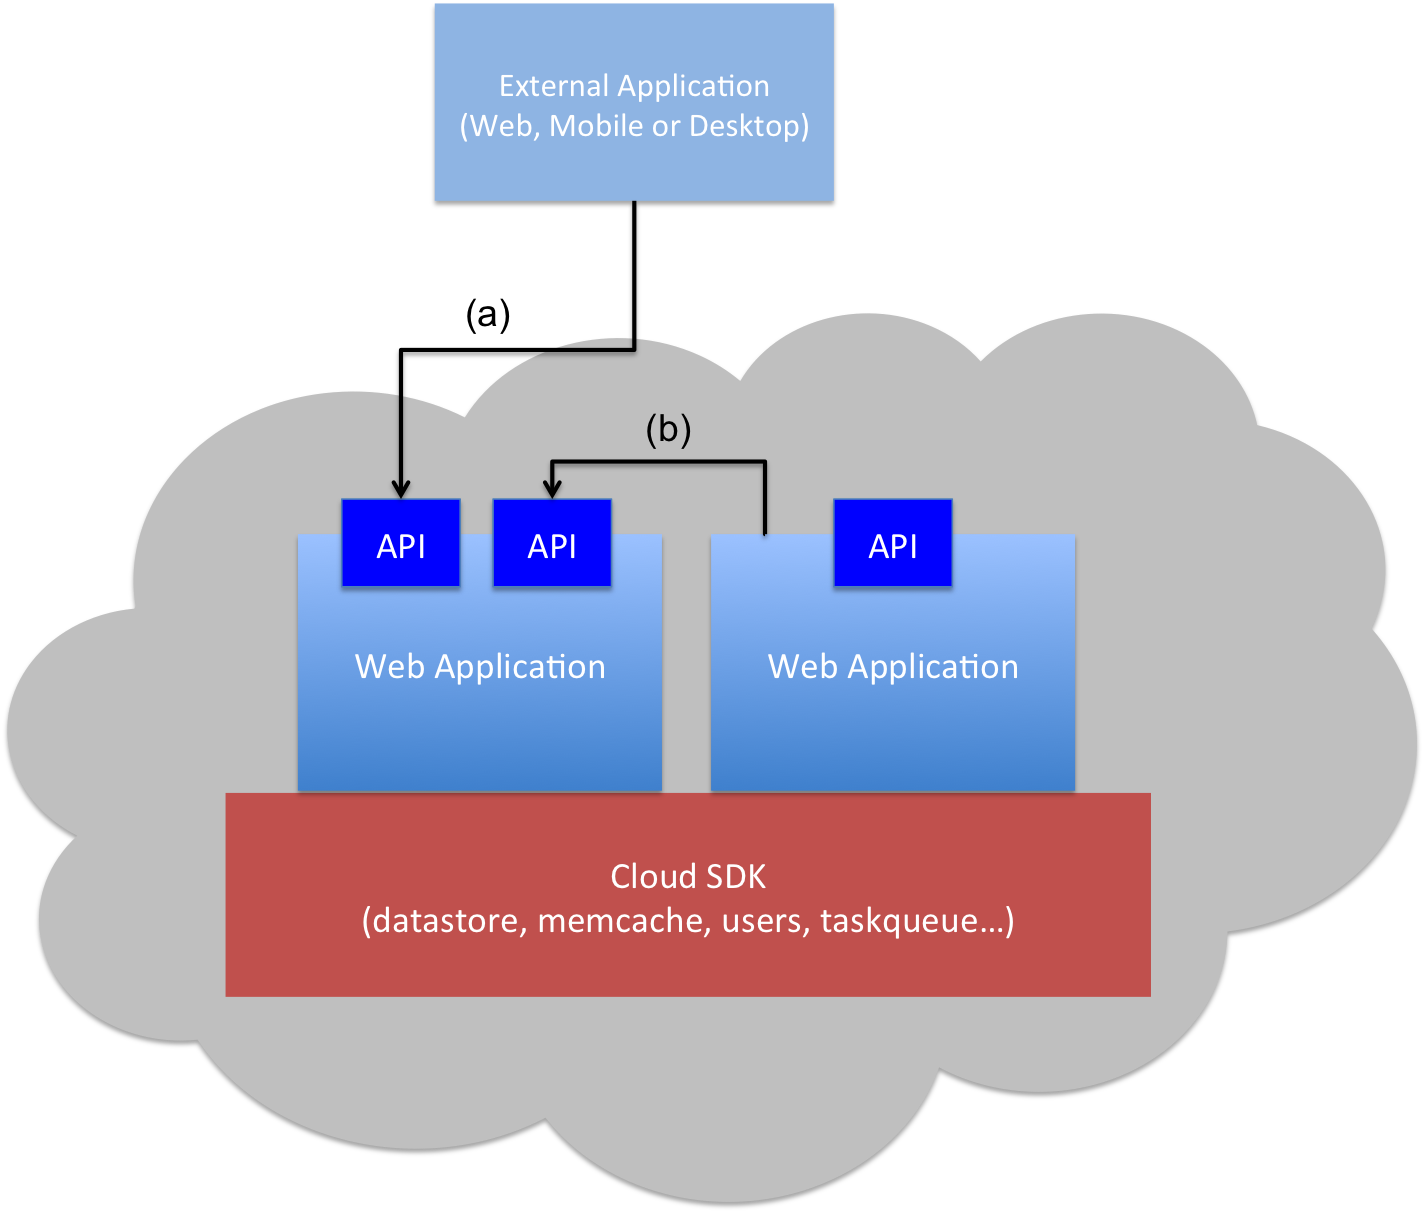
\includegraphics[scale=0.35]{cloud_app_model}
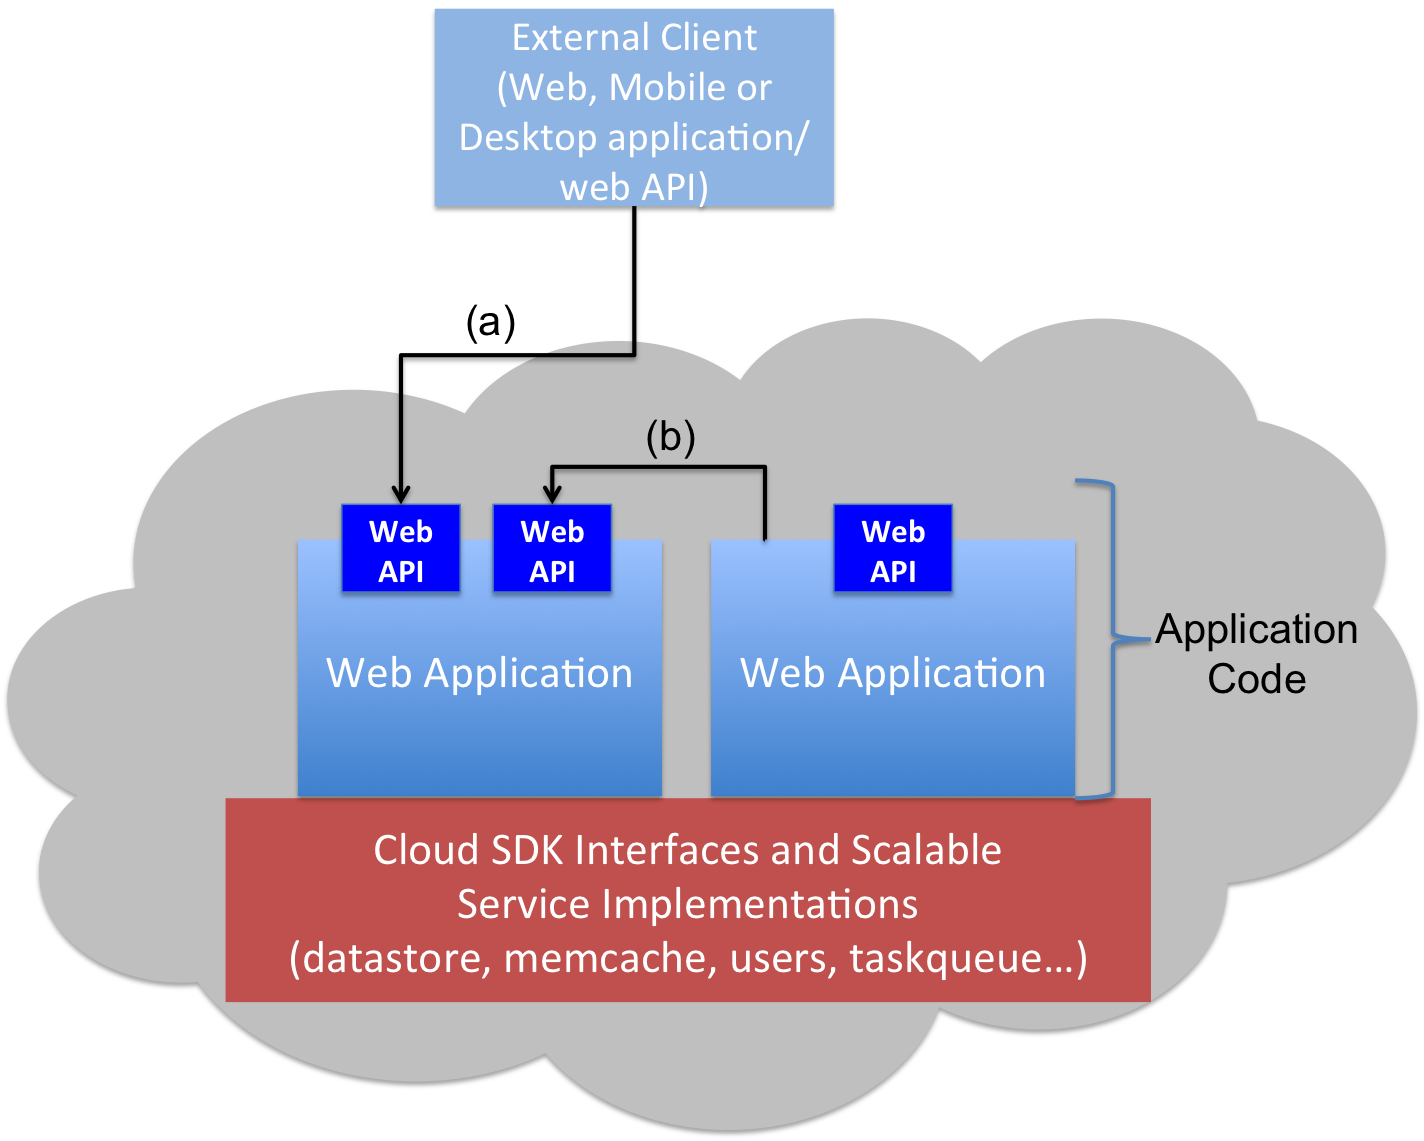
\includegraphics[scale=0.35]{sdk}
\caption{Web APIs deployed in a PaaS cloud: (a) An external client invoking 
a PaaS-hosted web API;
(b) A Paas-hosted web API invoking a web API hosted in the same cloud.}
\label{fig:cloud_app_model}
\end{figure}

Figure~\ref{fig:cloud_app_model} illustrates the PaaS deployment model for web APIs.
Developers implement their applications using a combination of operations
from the cloud SDK and their own code.  The service implementations for the 
cloud SDK are highly scalable, highly available (have SLAs associated with them),
and automatically managed and connected to the web API by the platform.
Web APIs that run in PaaS clouds can be accessed by external or co-located clients.
Clients can be other web APIs, applications, and users via their browsers.

Typically, \textit{all} PaaS-hosted web APIS implement one or more
cloud SDK calls.  The reason for this is two-fold.  First, 
cloud SDKs provide web APIs with much of the functionality that they require.
Second, PaaS clouds ``sandbox'' web APIs to enforce quotas/billing
and to restrict certain functionality
(e.g. local file system access, direct memory access, use of certain libraries, multi-threading) that can lead to security holes, platform instability, or scaling issues~\cite{gae-sandbox}.

The sandbox places other important restrictions on web APIs that additionally
simplify our analysis.
First, the only way to execute a PaaS-hosted web API is via HTTP/s (request-response 
pattern).  As a result, 
all web API operations start and end at well defined points in the program and 
structure can be inferred from the pattern.  Second,
concurrency is restricted by capping the number of threads
and requiring that a thread cannot outlive the request
that creates it.  Third, PaaS clouds enforce quotas and limits on service
(cloud SDK) use~\cite{azure-limits,gae-limits,gae-sandbox}.
App Engine for example, requires that all web API requests complete in 60 seconds (or they are terminated by the platform).  Such enforcement places a strict upper bound on the
execution of a web API operation (request response).

